% !Mode:: "TeX:UTF-8"
%此为章节二模板
%\chapter、\section、\subsection、\subsubsection分别对应一二三四级标题
\chapter{图片示例}\label{ch:2}

\section{图片排版示例}
\textbf{注意}:使用\textbackslash caption[]\{\}命令时,如果不需要设置缩写目录的内容,一定要删掉[],否则插图插表索引将不会显示该图或表的目录。

\textbf{建议}:在论文写作时图片位置可以先按照写作时的习惯进行放置,待到完成所有写作内容后再进行详细调整图片位置。

\subsection{图片格式}

\LaTeX 中图片推荐使用pdf格式。使用Origin可导出矢量无白边的图片以保证清晰度,其次推荐使用jpg,png格式图片。

为了保证图片的清晰,jpg图片导出时ppi建议设置为300,png图片导出时建议宽度设置为1024像素(可根据需求自行设置),长度随宽度变化。

\subsection{单图排版示例}

\begin{figure}[htb]
    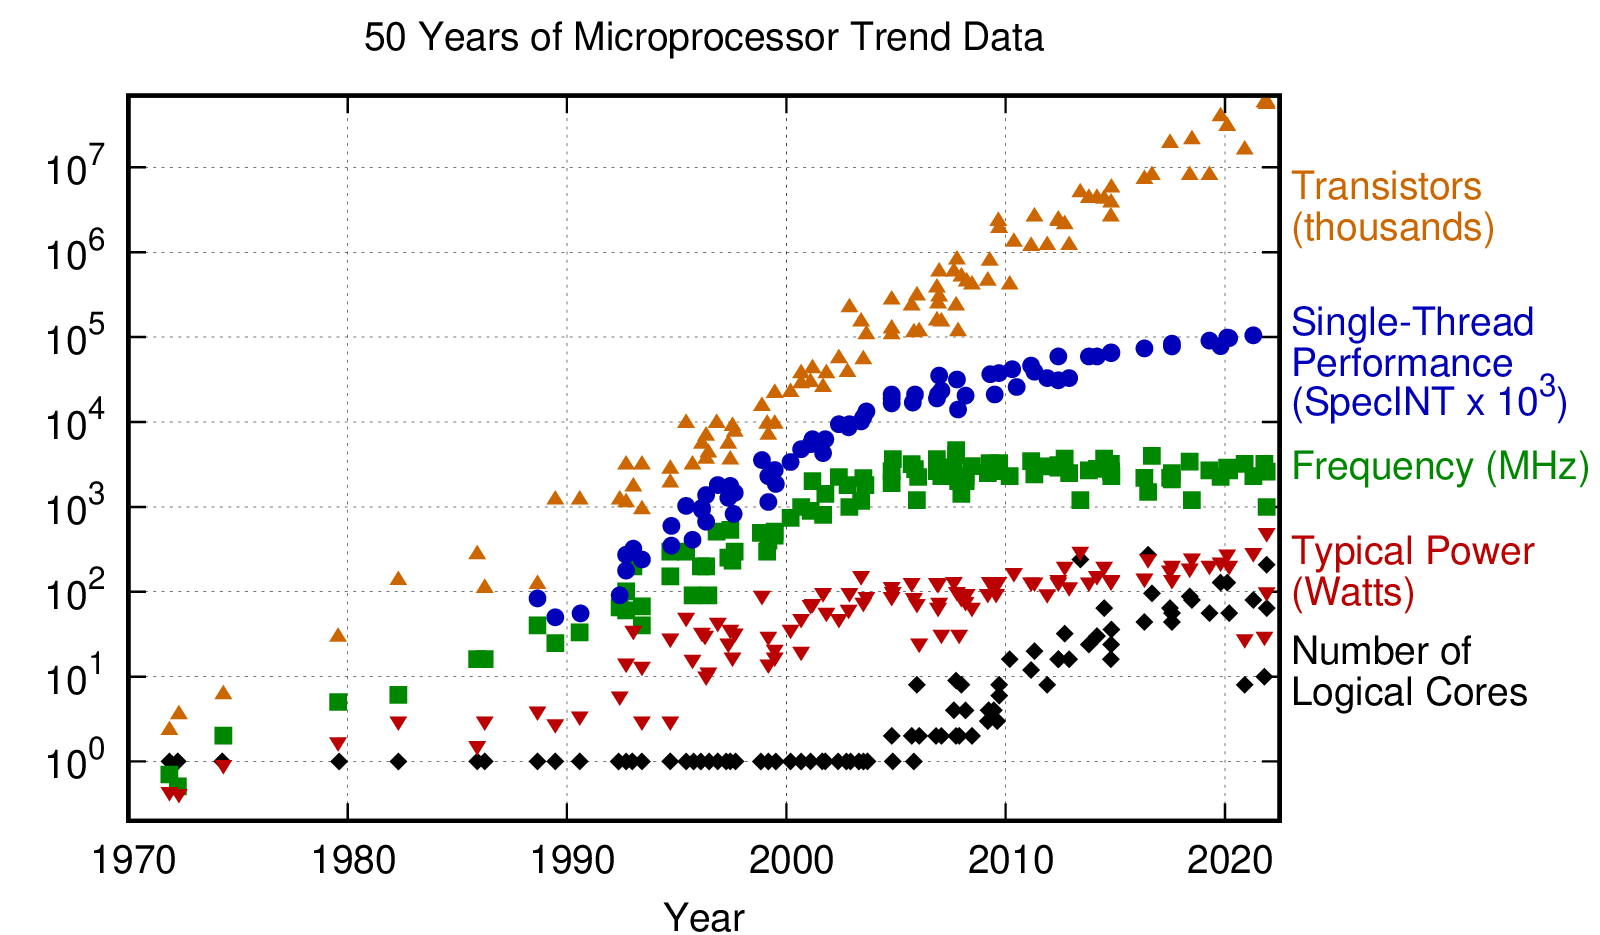
\includegraphics[width=0.8 \textwidth]{50-years-processor-trend.png}
    \caption[处理器发展]{近50年微处理器发展趋势} % 中括号中内容为插图索引中显示内容,可在题注内容过长时使用
    \label{fig:processor-trend}
\end{figure}

图片引用示例:\cref{fig:processor-trend}。

\subsection{多图排版示例}
同一行中的子图之间要留有空间,不要占满!否则会自动换行!

子图之间空一行表示换行。

插入子图请使用\textbackslash subfloat\{\}命令。

\begin{figure}[htb]
    \subfloat[改进前的结构]{
        \label{fig:Unimproved-cooling-structure}
        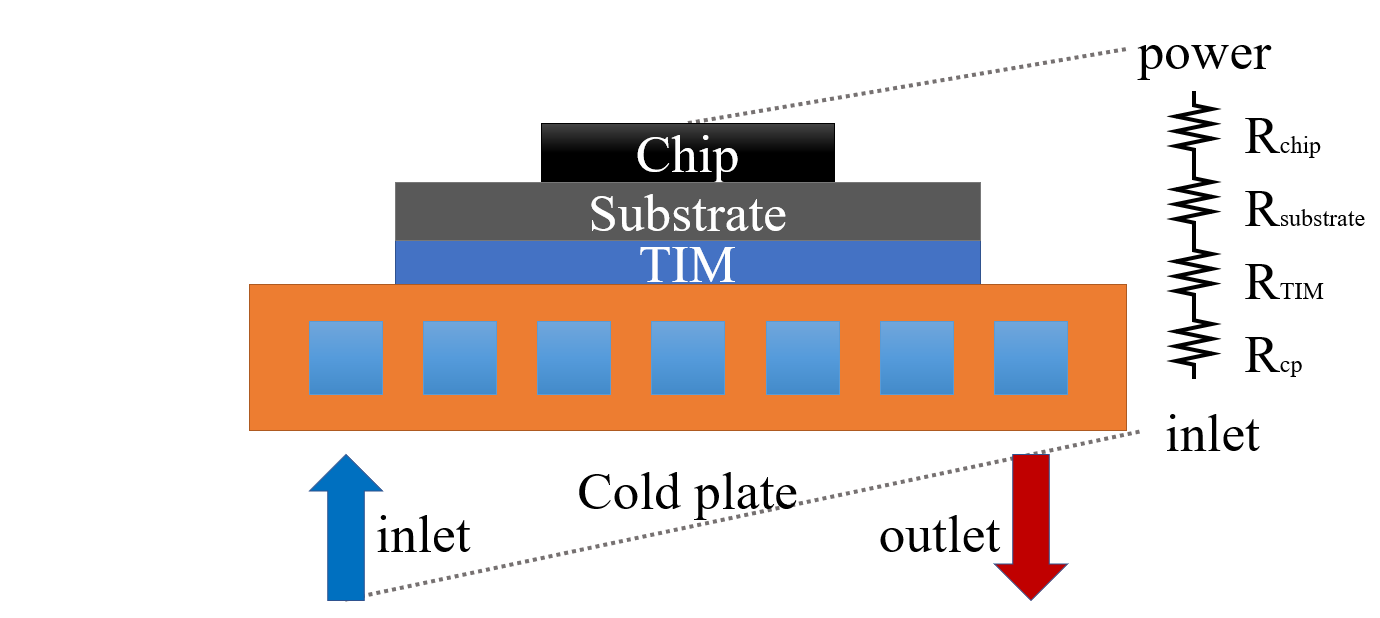
\includegraphics[width=0.45\linewidth]{Unimproved-cooling-structure.png}}
    \subfloat[基板内进行微通道散热]{
        \label{fig:LTCC-Microchannels}
        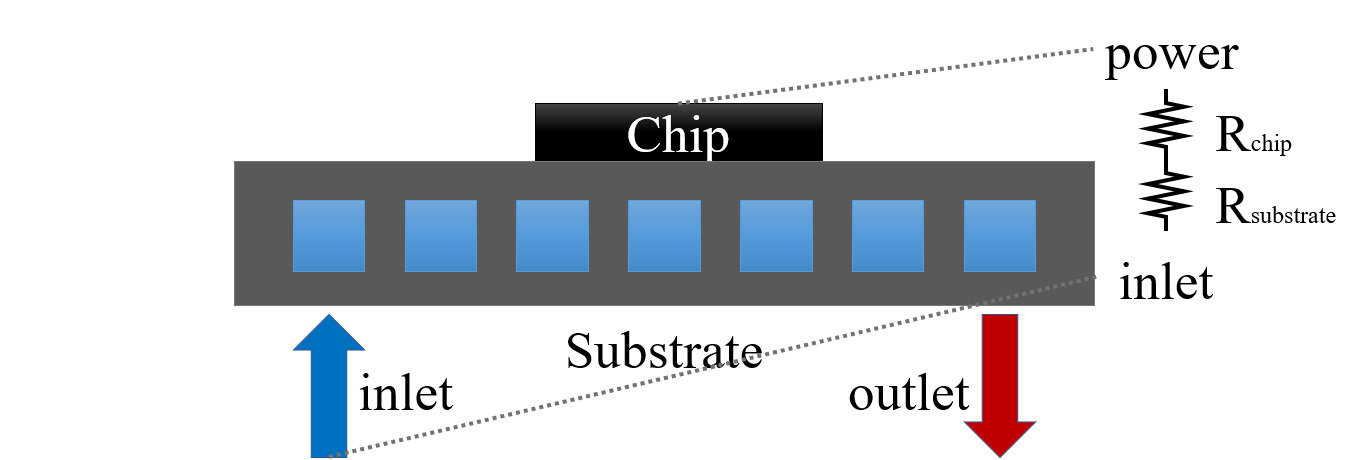
\includegraphics[width=0.45\linewidth]{LTCC-Microchannels.png}}

    \subfloat[嵌入散热模块]{
        \label{fig:Embedded-cooling-module}
        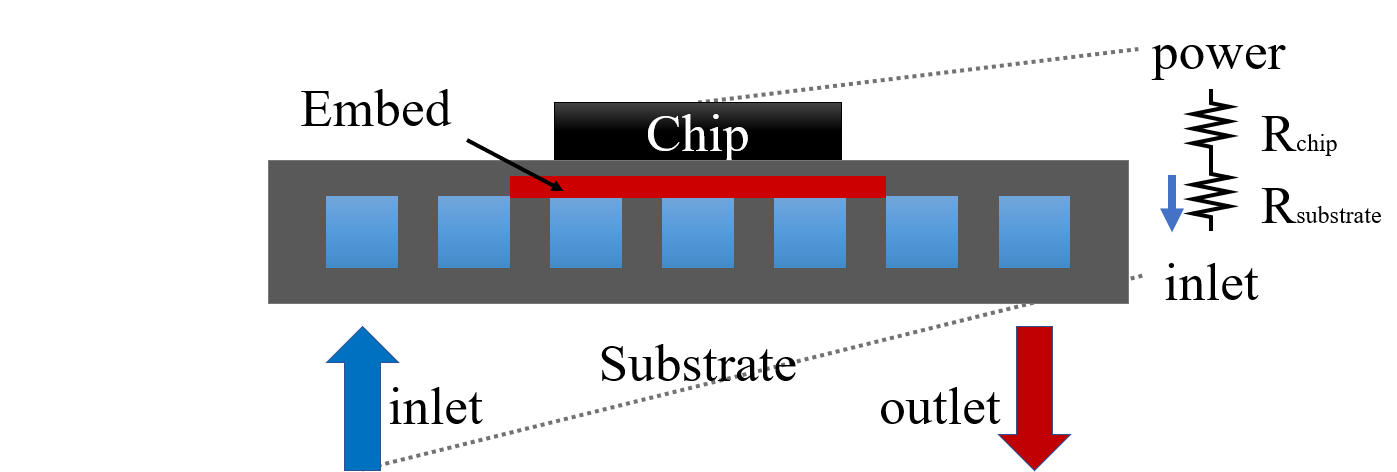
\includegraphics[width=0.45\linewidth]{Embedded-cooling-module.png}}
    \subfloat[带针鳍或肋的嵌入式散热模块]{
        \label{fig:Rib-pin-fin}
        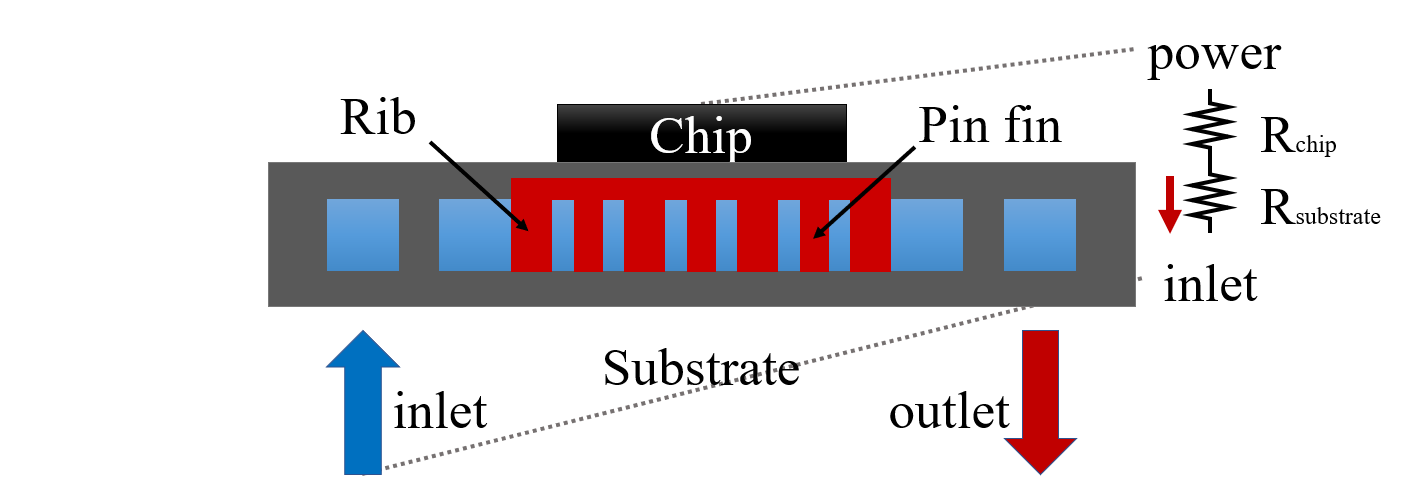
\includegraphics[width=0.45\linewidth]{Rib-pin-fin.png}}
    \caption{三种强化传热途径示意图}
    \label{fig:Three-enhanced-heat-transfer-paths}
\end{figure}

子图引用示例:\cref{fig:Unimproved-cooling-structure},

整图引用示例:\cref{fig:Three-enhanced-heat-transfer-paths}。

提供三种不同的Tikz绘图示例,分别为柱状图(存在问题是少一列,过几天修改),多点折线图,少点折线图(数据均已进行扰动,有空还是要大改一下数据)。

\begin{figure}
    \subfloat[生成证明\label{fig-2}]{
        \begin{tikzpicture}[global scale = 0.55]
            \begin{axis}[
                x tick label style={
                    /pgf/number format/1000 sep=.},
                y tick label style={
                    /pgf/number format/1000 sep=.},
                xlabel={参与者数量},
                ylabel={耗时 (ms)},
                ymin=0, ymax=1100,
                ybar=10pt,
                bar width=20pt,
                enlarge x limits={abs=6pt},
                legend cell align={left},
                enlarge y limits={value=0.1,upper},
                ybar interval=0.7,
                legend pos=north west,
                xtick=data,
                xticklabels={100, 200, 300, 400, 500},
                ytick={0, 500, 1000},
                legend style={font=\huge},
                label style={font=\huge},
                tick label style={font=\huge}
                ]
                \addplot[color=orange,fill=orange!50,bar shift=-6pt] coordinates {
                    (1,166.7)
                    (2,334.6)
                    (3,502.1)
                    (4,667.2)
                    (5,831.4)
                };
                \addplot[color=blue,fill=blue!50,bar shift=-2pt] coordinates {
                    (1,234.3)
                    (2,501.5)
                    (3,768.7)
                    (4,1035.9)
                    (5,1303.1)
                };
                \addplot[color=green,fill=green!50,bar shift=0pt] coordinates {
                    (1,265.824)
                    (2,533.074)
                    (3,800.234)
                    (4,1067.464)
                    (5,1334.614)
                };
                \addplot[color=gray,fill=gray!50,bar shift=2pt] coordinates {
                    (1,130.214)
                    (2,261.854)
                    (3,393.414)
                    (4,525.034)
                    (5,656.674)
                };
                \addplot[color=red,fill=red!50,bar shift=6pt] coordinates {
                    (1,117.529)
                    (2,236.439)
                    (3,343.239)
                    (4,470.919)
                    (5,588.179)
                };
                \legend{Xu et al.\cite{xu2019verifynet},Zhang et al.\cite{zhang2020privacy},Shen et al.\cite{shen2018enabling},Han et al.\cite{han2022verifiable},本方案}
            \end{axis}
        \end{tikzpicture}
    }
    \hfill
    \subfloat[验证证明\label{fig-3}]{
        \begin{tikzpicture}[global scale = 0.55]
            \begin{axis}[
                x tick label style={
                    /pgf/number format/1000 sep=.},
                y tick label style={
                    /pgf/number format/1000 sep=.},
                xlabel={参与者数量},
                ylabel={耗时 (ms)},
                ymin=0, ymax=2700,
                ybar=10pt,
                bar width=20pt,
                enlarge x limits={abs=6pt},
                legend cell align={left},
                enlarge y limits={value=0.1,upper},
                ybar interval=0.7,
                legend pos=north west,
                xtick=data,
                xticklabels={100, 200, 300, 400, 500},
                legend style={font=\huge},
                label style={font=\huge},
                tick label style={font=\huge}
                ]
                \addplot[color=orange,fill=orange!50,bar shift=-6pt] coordinates {
                    (1,216.316)
                    (2,291.916)
                    (3,362.116)
                    (4,431.616)
                    (5,502.716)
                };
                \addplot[color=blue,fill=blue!50,bar shift=-10pt] coordinates {
                    (1,1169.397)
                    (2,1436.597)
                    (3,1703.797)
                    (4,1970.997)
                    (5,2238.197)
                };
                \addplot[color=green,fill=green!50,bar shift=-5pt] coordinates {
                    (1,361.874)
                    (2,629.074)
                    (3,896.274)
                    (4,1163.474)
                    (5,1430.674)
                };
                \addplot[color=gray,fill=gray!50,bar shift=5pt] coordinates {
                    (1,779.338)
                    (2,1445.338)
                    (3,2111.338)
                    (4,2777.338)
                    (5,3443.338)
                };
                \addplot[color=red,fill=red!50,bar shift=10pt] coordinates {
                    (1,80.632)
                    (2,160.932)
                    (3,241.232)
                    (4,321.532)
                    (5,401.832)
                };
                \legend{XXX et al.\cite{Lau_2022},YYY et al.\cite{Lau_2022},ZZZ et al.\cite{Lau_2022},HHH et al.\cite{Lau_2022},本方案}
            \end{axis}
        \end{tikzpicture}
    }
    \caption[方案一的开销比较]{比较结果 (a) 生成证明的计算开销比较 (b)验证的计算开销比较(在\cref{fig-3}中,Zhang 等人的方案中的 $d=25$~\cite{zhang2020privacy} 和 Shen 等人的方案中的 $l=10$\cite{shen2018enabling})}
    \label{fig3}
\end{figure}

在\cref{fig-2}和\cref{fig-3}中,是引用。

\begin{figure}[tbh!]
    \subfloat[MNIST\label{fig-4}]{
        \begin{tikzpicture}[global scale = 0.6]
            \begin{axis}[
                xlabel={迭代次数},
                ylabel={准确率 (\%)},
                xticklabel style={anchor= east,rotate=45 },
                xmax=250,
                xmin=0,
                ymax=100,
                ymin=38,
                legend pos=south east,
                ymajorgrids=true,
                grid style=dashed,
                legend style={nodes={scale=1, transform shape}},
                legend style={font=\huge},
                label style={font=\huge},
                tick label style={font=\huge}
                ]
                \addplot[
                color=blue,
                mark=.,
                only marks,
                sharp plot,
                line width=1.5pt
                ] table [x index=0, y index=1] {Data/data_sub_2.dat};
                \addplot[
                color=green,
                mark=.,
                only marks,
                sharp plot,
                line width=1.5pt
                ] table [x index=0, y index=2] {Data/data_sub_2.dat};
                \addplot[
                color=red,
                mark=.,
                only marks,
                sharp plot,
                line width=1.5pt
                ] table [x index=0, y index=3] {Data/data_sub_2.dat};
                \legend{100 参与者, 300 参与者, 500 参与者}
            \end{axis}
        \end{tikzpicture}
    }
    \hfill
    \subfloat[CIFSAR{\footnotesize 100}\label{fig-5}]{
        \begin{tikzpicture}[global scale = 0.6]
            \begin{axis}[
                xlabel={迭代次数},
                ylabel={准确率 (\%)},
                xticklabel style={anchor= east,rotate=45 },
                xmax=250,
                xmin=0,
                ymax=80,
                ymin=23,
                legend pos=south east,
                ymajorgrids=true,
                grid style=dashed,
                legend style={nodes={scale=1, transform shape}},
                legend style={font=\huge},
                label style={font=\huge},
                tick label style={font=\huge}
                ]
                \addplot[
                color=blue,
                mark=.,
                only marks,
                sharp plot,
                line width=1.5pt
                ] table [x index=0, y index=1] {Data/data_sub_1.dat};
                \addplot[
                color=green,
                mark=.,
                only marks,
                sharp plot,
                line width=1.5pt
                ] table [x index=0, y index=2] {Data/data_sub_1.dat};
                \addplot[
                color=red,
                mark=.,
                only marks,
                sharp plot,
                line width=1.5pt
                ] table [x index=0, y index=3] {Data/data_sub_1.dat};
                \legend{100 参与者, 300 参与者, 500 参与者}
            \end{axis}
        \end{tikzpicture}
    }
    \caption[方案一的准确度与迭代次数关系]{不同数量的客户端的准确性与迭代次数的关系}
    \label{exp1}
\end{figure}

\begin{figure}[tbh!]
    \subfloat[MNIST\label{fig-6}]{
        \begin{tikzpicture}[global scale = 0.6]
            \begin{axis}[
                xlabel={参与者数量},
                ylabel={准确率 (\%)},
                symbolic x coords = {100,200,300,400,500},
                xticklabel style={anchor= east,rotate=45 },
                xtick=data,
                ymax=100,
                ymin=40,
                legend pos=south east,
                legend cell align={left},
                ymajorgrids=true,
                grid style=dashed,
                legend style={nodes={scale=1, transform shape}},
                legend style={font=\huge},
                label style={font=\huge},
                tick label style={font=\huge}
                ]
                \addplot+[mark size=3pt]
                coordinates {
                    (100, 91.0349)
                    (200, 91.7635)
                    (300, 92.1530)
                    (400, 93.5713)
                    (500, 94.2747)
                };\label{6c0}%原始
                \addplot+[mark size=3pt]
                coordinates {
                    (100, 88.4214)
                    (200, 88.6571)
                    (300, 89.5672)
                    (400, 90.6631)
                    (500, 91.2861)
                };\label{6c1}%Xu
                \addplot+[mark size=3pt]
                coordinates {
                    (100, 86.8072)
                    (200, 87.0289)
                    (300, 88.9112)
                    (400, 89.7785)
                    (500, 90.0550)
                };\label{6c2}%Zhang
                \addplot+[mark size=3pt]
                coordinates {
                    (100, 90.5275)
                    (200, 90.1048)
                    (300, 91.8314)
                    (400, 92.4257)
                    (500, 93.5617)
                };\label{6c3}%Shen
                \addplot+[mark size=3pt]
                coordinates {
                    (100, 91.2241)
                    (200, 91.7189)
                    (300, 92.6760)
                    (400, 93.1523)
                    (500, 93.8426)
                };\label{6c4}%Han
                \addplot+[mark size=3pt]
                coordinates {
                    (100, 86.4234)
                    (200, 88.3281)
                    (300, 89.5347)
                    (400, 90.2071)
                    (500, 91.8193)
                };\label{6c5}%5%
                \addplot+[mark size=3pt]
                coordinates {
                    (100, 82.6479)
                    (200, 85.4558)
                    (300, 87.1009)
                    (400, 88.3564)
                    (500, 89.6152)
                };\label{6c6}%10%
                \addplot+[mark size=3pt]
                coordinates {
                    (100, 73.4036)
                    (200, 76.6815)
                    (300, 77.5426)
                    (400, 78.1326)
                    (500, 78.9213)
                };\label{6c7}%20%
            \legend{本方案, XXX et al.\cite{Lau_2022}, YYY et al.\cite{Lau_2022}, ZZZ et al.\cite{Lau_2022}, HHH et al.\cite{Lau_2022}, 5\% 恶意参与者, 10\% 恶意参与者, 20\% 恶意参与者}
            \end{axis}
        \end{tikzpicture}
    }
    \hfill
    \subfloat[CIFSAR{\footnotesize 100}\label{fig-7}]{
        \begin{tikzpicture}[global scale = 0.6]
            \begin{axis}[
                %title={},
                xlabel={参与者数量},
                ylabel={准确率 (\%)},
                symbolic x coords = {100,200,300,400,500},
                xticklabel style={anchor= east,rotate=45 },
                xtick=data,
                ymax=80,
                ymin=20,
                legend pos=south east,
                legend cell align={left},
                ymajorgrids=true,
                grid style=dashed,
                legend style={nodes={scale=1, transform shape}},
                legend style={font=\huge},
                label style={font=\huge},
                tick label style={font=\huge}
                ]
                \addplot+[mark size=3pt]
                coordinates {
                    (100, 73.0039)
                    (200, 73.4271)
                    (300, 73.7160)
                    (400, 74.2513)
                    (500, 75.0248)
                };%原始
                \addplot+[mark size=3pt]
                coordinates {
                    (100, 70.5137)
                    (200, 71.2461)
                    (300, 71.5914)
                    (400, 72.6225)
                    (500, 73.3046)
                };%Xu
                \addplot+[mark size=3pt]
                coordinates {
                    (100, 70.0164)
                    (200, 71.2286)
                    (300, 72.1332)
                    (400, 72.4517)
                    (500, 73.1561)
                };%Zhang
                \addplot+[mark size=3pt]
                coordinates {
                    (100, 72.3538)
                    (200, 72.6216)
                    (300, 73.8918)
                    (400, 74.2905)
                    (500, 74.1621)
                };%Shen
                \addplot+[mark size=3pt]
                coordinates {
                    (100, 72.1013)
                    (200, 73.5135)
                    (300, 73.9425)
                    (400, 74.7297)
                    (500, 75.2756)
                };%Han
                \addplot+[mark size=3pt]
                coordinates {
                    (100, 68.5217)
                    (200, 70.4832)
                    (300, 71.7219)
                    (400, 72.0186)
                    (500, 72.3318)
                };%5%
                \addplot+[mark size=3pt]
                coordinates {
                    (100, 62.2815)
                    (200, 65.8233)
                    (300, 67.6183)
                    (400, 68.1124)
                    (500, 69.5276)
                };%10%
                \addplot+[mark size=3pt]
                coordinates {
                    (100, 53.6133)
                    (200, 55.5052)
                    (300, 58.4218)
                    (400, 61.1081)
                    (500, 62.3716)
                };%20%
                \legend{本方案, XXX et al.\cite{Lau_2022}, YYY et al.\cite{Lau_2022}, ZZZ et al.\cite{Lau_2022}, HHH et al.\cite{Lau_2022}, 5\% 恶意参与者, 10\% 恶意参与者, 20\% 恶意参与者}
            \end{axis}
        \end{tikzpicture}
    }
    \caption[方案一的准确度比较]{准确度比较}
    \label{exp2}
\end{figure}

引用也是一样的,如\cref{fig-4}和\cref{fig-5}。和\cref{fig-6}和\cref{fig-7}。以及对整个图的引用\cref{exp1}和\cref{exp2}。

\section{本章小节}
本章介绍了基于嵌入式散热模块的微通道散热技术所涉及的基……